% Competing research AND competing analyses: truth feeds three studies with
% different findings, each study feeds three policy analyses, and each policy
% maker picks the one analysis that suits them. Redrawn in the style of
% evidence-to-policy.tex from the dissertation figure
% (dissertation-manuscript/dissertation.tex, around line 687). Built by
% ./build.sh as the "competing-research" variant.

\documentclass[border=10pt,tikz]{standalone}
\usepackage{tikz}
\usetikzlibrary{positioning,shapes.geometric,decorations.pathreplacing,calc}
\pdftrailerid{}

\begin{document}
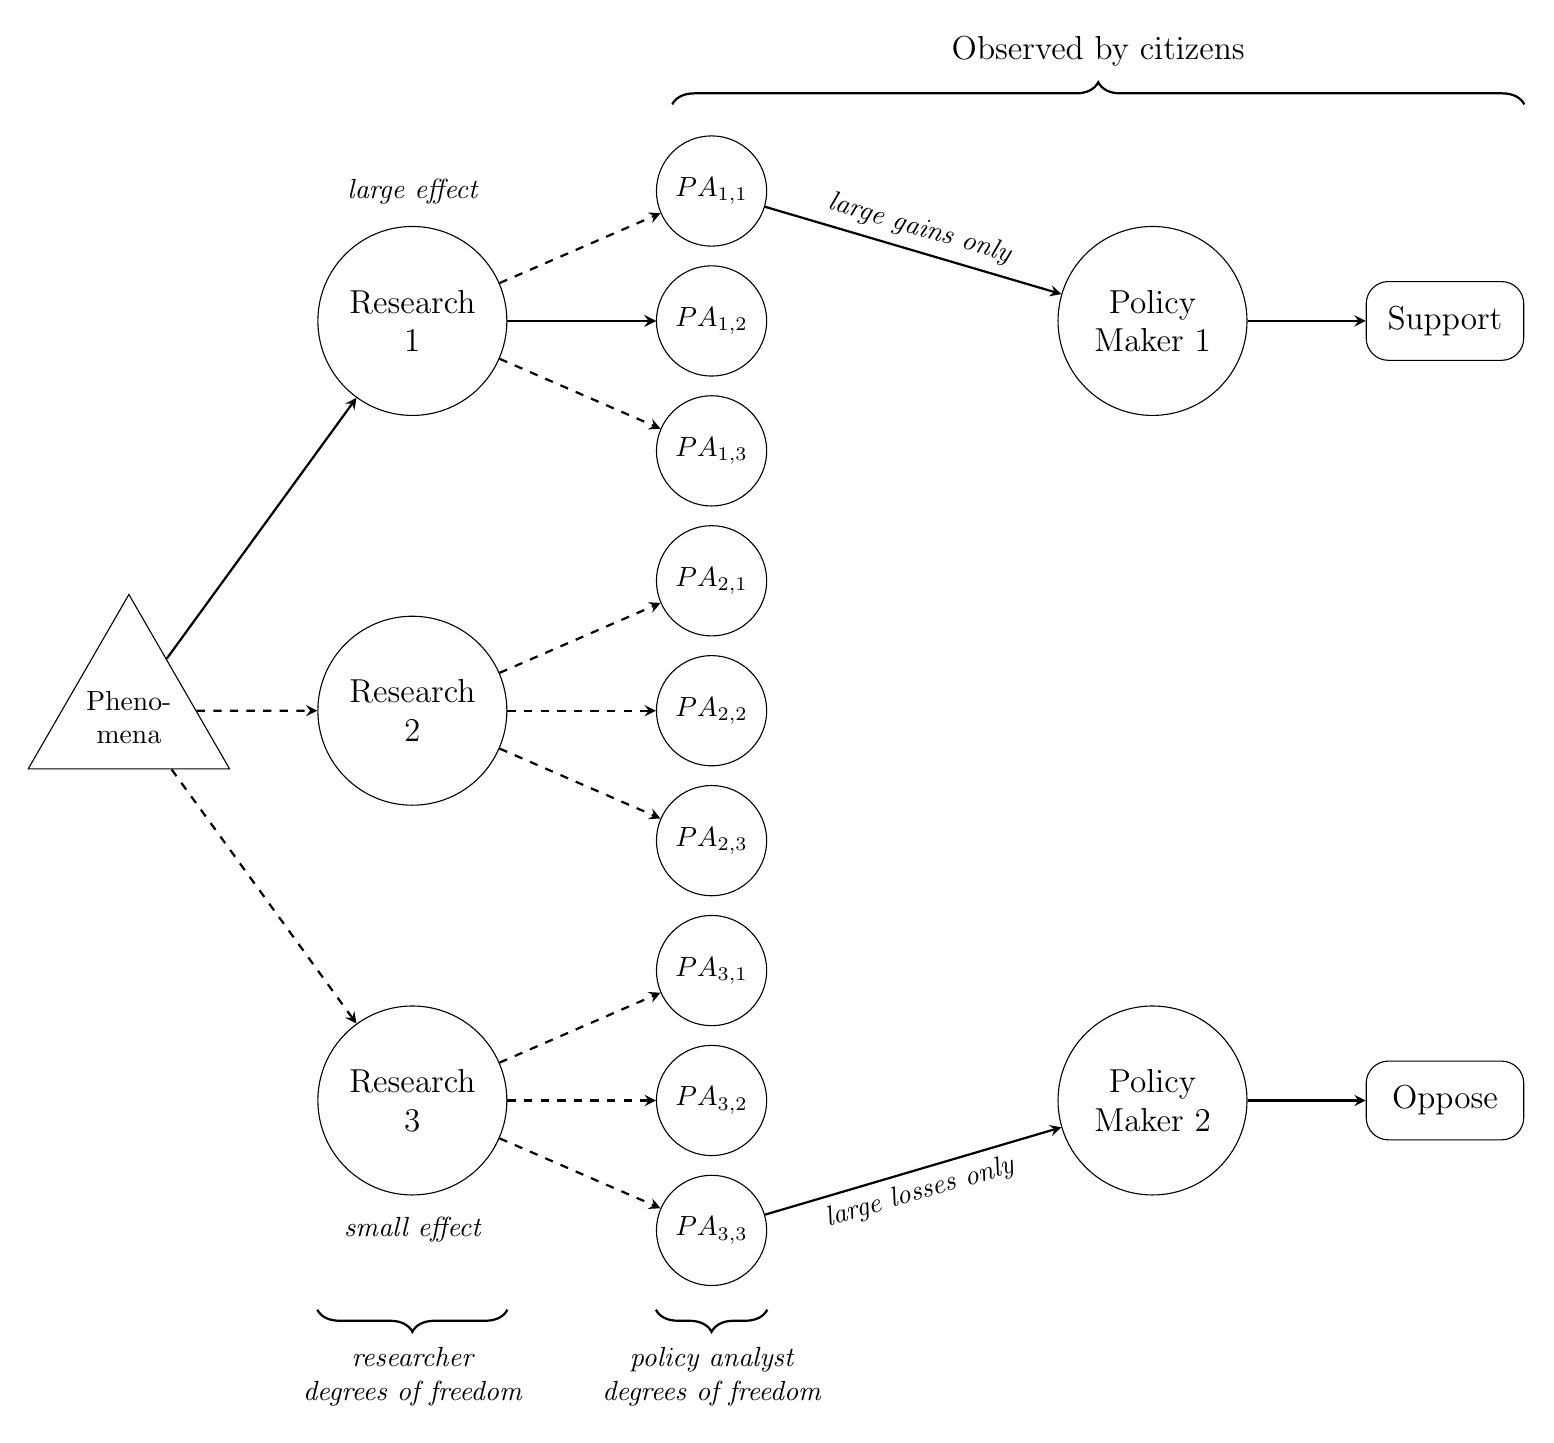
\begin{tikzpicture}[
  every node/.style={font=\large},
  bigcirc/.style={circle, draw, minimum size=2.4cm, align=center, inner sep=2pt},
  smallcirc/.style={circle, draw, minimum size=1.4cm, inner sep=1pt, font=\normalsize},
  tri/.style={regular polygon, regular polygon sides=3, draw,
              minimum size=2.5cm, align=center, inner sep=0pt},
  rrect/.style={rectangle, rounded corners=8pt, draw, minimum width=2cm,
                minimum height=1cm, align=center},
  arr/.style={-stealth, thick},
  darr/.style={-stealth, thick, dashed},
  note/.style={font=\normalsize\itshape, align=center},
  brace/.style={decorate, decoration={brace, amplitude=8pt}, thick},
  mbrace/.style={decorate, decoration={brace, mirror, amplitude=8pt}, thick}
]

% Vertical layout: 9 analyses 1.65cm apart; each study sits level with the
% middle analysis of its group.
\def\pitch{1.65}

% Phenomena: an empty triangle with the label placed as its own node, low in
% the triangle where it is widest, so the hyphenated label fits inside and the
% triangle keeps the size (and the layout) it had with a one-word label: an
% invisible \phantom{Truth} sizes it exactly as the old visible label did.
\node[tri] (T) at (0,0) {\phantom{Truth}};
\node[align=center, inner sep=0pt, anchor=south, font=\normalsize] at ($(T.corner 2)!0.5!(T.corner 3)+(0,9pt)$) {Pheno-\\mena};
\foreach \g in {1,2,3} {
  \node[bigcirc] (R\g) at (3.6, {(2-\g)*3*\pitch}) {Research\\\g};
  \foreach \j in {1,2,3}
    \node[smallcirc] (PA\g\j) at (7.4, {(2-\g)*3*\pitch + (2-\j)*\pitch}) {$PA_{\g,\j}$};
}
\node[bigcirc] (PM1) at (13.0,  {3*\pitch}) {Policy\\Maker 1};
\node[bigcirc] (PM2) at (13.0, {-3*\pitch}) {Policy\\Maker 2};
\node[rrect, right=1.5cm of PM1] (S) {Support};
\node[rrect, right=1.5cm of PM2] (O) {Oppose};

\node[note, above=0.15cm of R1] {large effect};
\node[note, below=0.15cm of R3] {small effect};

% Phenomena to research: one solid path, the others possible.
\draw[arr]  (T) -- (R1);
\draw[darr] (T) -- (R2);
\draw[darr] (T) -- (R3);

% Research to analysis: every analysis is possible, one path is solid.
\foreach \g in {1,2,3}
  \foreach \j in {1,2,3}
    \draw[darr] (R\g) -- (PA\g\j);
\draw[arr] (R1) -- (PA12);

% Each policy maker takes the analysis that suits them.
\draw[arr] (PA11) -- node[note, above, sloped] {large gains only} (PM1);
\draw[arr] (PA33) -- node[note, below, sloped] {large losses only} (PM2);
\draw[arr] (PM1) -- (S);
\draw[arr] (PM2) -- (O);

% What citizens see, and where the degrees of freedom sit.
\coordinate (top) at ($(PA11.north west)+(0,0.6)$);
\draw[brace] (top) -- (top -| S.east) node[midway, above=10pt] {Observed by citizens};
\coordinate (bot) at ($(PA33.south)+(0,-0.3)$);
\draw[mbrace] (R3.west |- bot) -- (R3.east |- bot)
  node[midway, below=10pt, note] {researcher\\degrees of freedom};
\draw[mbrace] (PA33.west |- bot) -- (PA33.east |- bot)
  node[midway, below=10pt, note] {policy analyst\\degrees of freedom};

\end{tikzpicture}
\end{document}
